
\section{\label{sec:tutorial:shearwave:hex8}3D Bar Discretized with Hexahedra}

PyLith features discussed in this tutorial:
\begin{itemize}
\item Dynamic solution
\item CUBIT mesh format
\item Absorbing dampers boundary conditions
\item Kinematic fault interface conditions
\item Elastic isotropic linearly elastic material
\item VTK output
\item Linear hexahedral cells
\item SimpleDB spatial database
\item ZeroDispDB spatial database
\end{itemize}
All of the files necessary to run the examples are contained in the
directory \texttt{examples/bar\_shearwave/hex8.}


\subsection{Mesh Generation}

The mesh is a simple rectangular prism 8 km by 400 m by 400 m (Figure
\ref{fig:shearwave:hex8:mesh}). This mesh could be generated via
a simple script, but it is even easier to generate this mesh using
CUBIT. We provide documented CUBIT journal files in \texttt{examples/bar\_shearwave/hex8.}
We first create the geometry, mesh the domain using hexahedral cells,
and then create blocks and nodesets associated with the materials
and boundary conditions.

\noindent \begin{center}
\begin{figure}
\begin{centering}
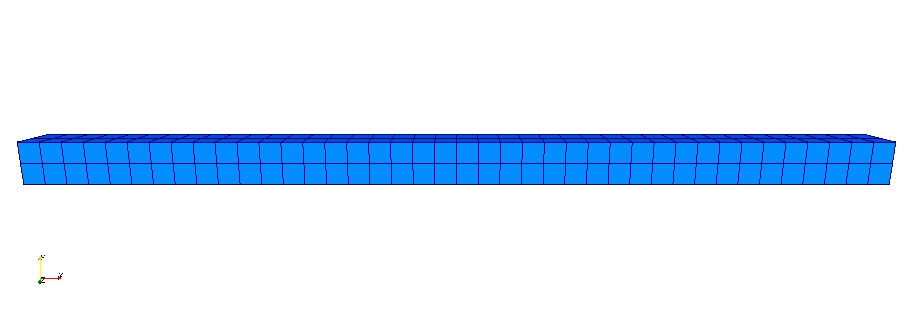
\includegraphics[scale=0.5]{tutorials/shearwave/figs/hex8mesh}
\par\end{centering}

\caption{Mesh composed of hexahedral cells generated by CUBIT used for the
example problem.\label{fig:shearwave:hex8:mesh}}
\end{figure}

\par\end{center}


\subsection{Simulation Parameters}

The simulation parameters match those in the tri3 and tet4 examples.
As in the tet4 example, we fix both the longitudinal degree of freedom
and the out-of-plane transverse degree of freedom. Using eight-point
quadrature permits use of a time step of 1/20 s, which is slightly
larger than the time step of 1/30 s used in the tri3 and tet4 simulations.
All of the parameters are set in the \texttt{pylithapp.cfg} file.
To run the problem, simply run PyLith without any command line arguments:
\begin{lyxcode}
pylith
\end{lyxcode}
The VTK files will be written to the \texttt{output} directory. The
output includes the displacement and velocity fields over the entire
domain at every other time step (0.10 s), the slip and change in traction
vectors on the fault surface in along-strike and normal directions
at every other time step (0.10 s), and the strain and stress tensors
for each cell at every 20th time step (1.0 s). If the problem ran
correctly, you should be able to generate a figure such as Figure
\ref{fig:shearwave:hex8:deform}, which was generated using ParaView.

\noindent \begin{center}
\begin{figure}
\begin{centering}
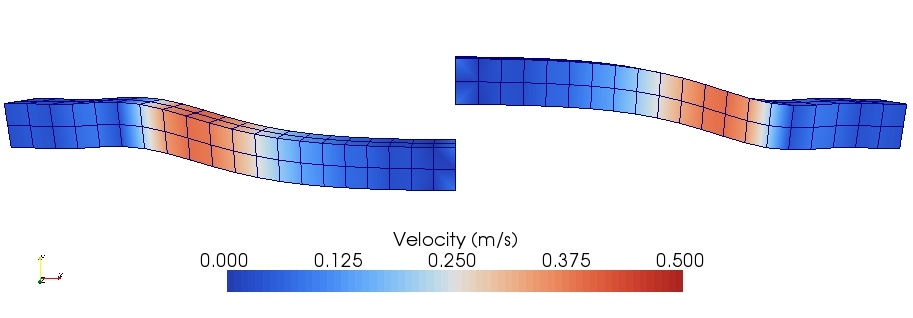
\includegraphics[scale=0.5]{tutorials/shearwave/figs/hex8deform30}
\par\end{centering}

\caption{Displacement field in the bar at 3.0 s. Deformation has been exaggerated
by a factor of 800.\label{fig:shearwave:hex8:deform}}
\end{figure}

\par\end{center}
